% Preamble
% ---
\documentclass{article}


% Packages
% ---
%\usepackage{amsmath} % Advanced math typesetting
\usepackage[utf8]{inputenc} % Unicode support (Umlauts etc.)
\usepackage[italian]{babel} % Change hyphenation rules
\usepackage{hyperref} % Add a link to your document
\usepackage{graphicx} % Add pictures to your document
\usepackage{listings} % Source code formatting and highlighting
\usepackage{caption}
\usepackage{subcaption}

% custom commands
\newcommand{\quotes}[1]{``#1''}

\graphicspath{ {./img/} }

\begin{document}

    \author{Federico Rachelli}
    \title{\vspace{-2cm}DataVirus.it}
    \maketitle

    L'app \textbf{\href{https://datavirus.it}{DataVirus.it}} é una implementazione Android del sito web omonimo.
    Fornisce all'utente una visualizzazione grafica dei dati del Dipartimento di Protezione Civile sull'andamento dell'epidemia di COVID-19.
    \\
    I dati sono accedibili dal \href{https://github.com/pcm-dpc/COVID-19}{repository GitHub ufficiale} della Protezione Civile. 
    Tali dati vengono aggiornati a cadenza giornaliera (a partire dalle ore 18:00) fino alla fine dello stato di emergenza dichiarato dal Consiglio dei Ministri in data 31 Gennaio 2020.
    \\
    Per riferimenti precisi sul codice si prega di controllare il Javadoc fornito con la documentazione ed il codice dell'app.
    
    \section{Visualizzazione dati}
    L'applicazione all'avvio visualizza una schermata di caricamento dei dati dal Dipartimento di Protezione Civile. 
    Tali dati, una volta ottenuti, sono elaborati e vengono mostrati all'utente gli andamenti a livello nazionale dell'epidemia (Figura \ref{fig1:sub1}).
    
    \begin{figure}[h]
        \centering
        \begin{subfigure}{.5\textwidth}
          \centering
          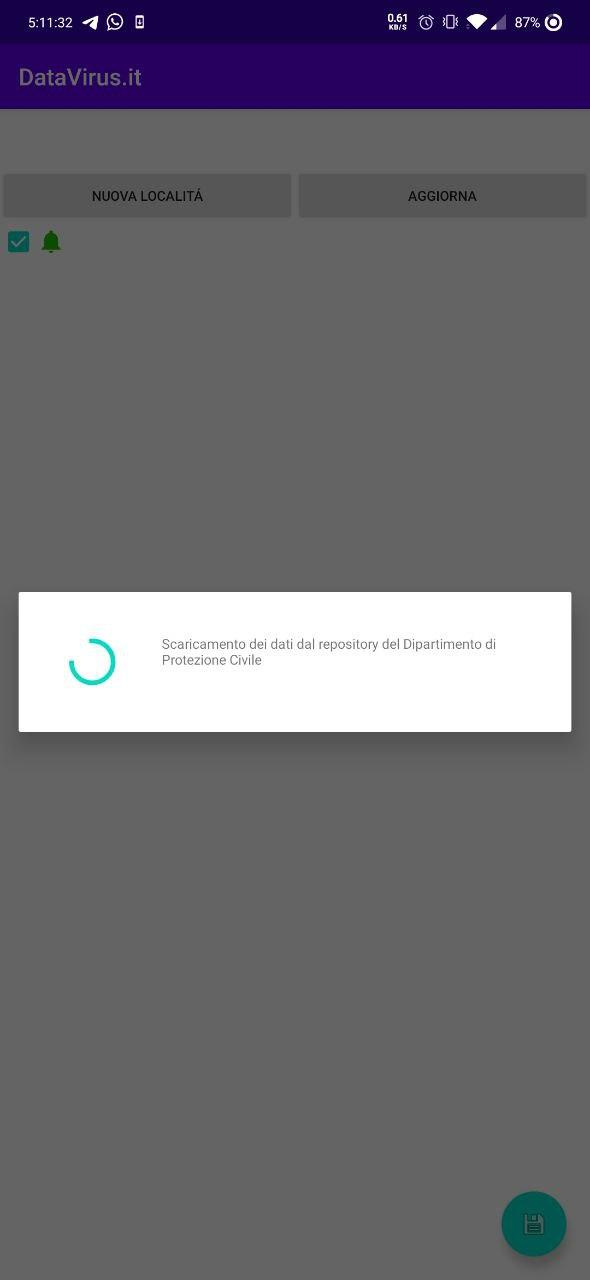
\includegraphics[width=.8\linewidth]{loading_dialog.jpg}
          \caption{Caricamento dei dati}
          \label{fig1:sub1}
        \end{subfigure}%
        \begin{subfigure}{.5\textwidth}
          \centering
          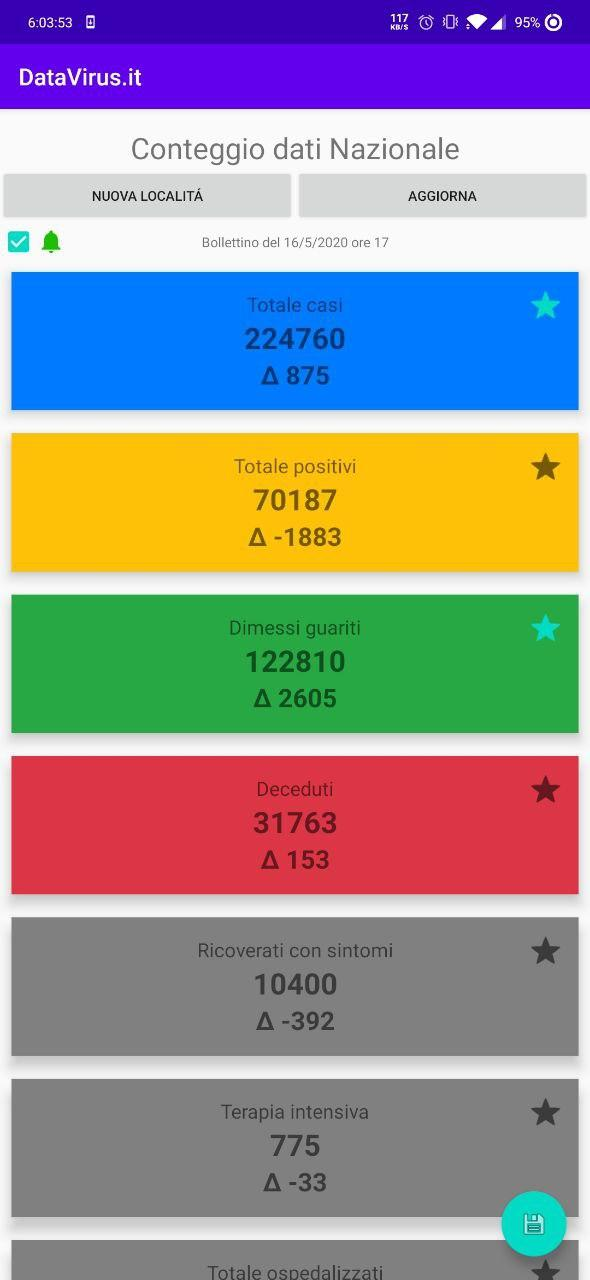
\includegraphics[width=.8\linewidth]{main_activity.jpg}
          \caption{Andamento nazionale}
          \label{fig1:sub2}
        \end{subfigure}
    \end{figure}
    
    Come si puó notare nella figura \ref{fig1:sub2}, questa é la schermata principale dell'applicazione. 
    Viene mostrato in alto la denominazione territoriale dei dati (nella scermata principale verrá mostrato l'andamento nazionale). Sotto i pulsanti, viene visualizzata la data dell'ultimo aggiornamento disponibile dal Dipartimento di Protezione Civile.
    \\
    Il pulsante \quotes{Aggiorna} ricarica i dati dal repository.
    \\
    Vengono poi visualizzate le tile contenenti il dato odierno e la relativa variazione (delta) rispetto alla giornata precedente.
    \\
    \emph{Nota:} il Dipartimento di Protezione Civile (\textbf{DPC}) (ad oggi) fornisce solamente il dato riguardante il totale dei contagiati per tutte le province del territorio italiano.
    
    \subsection{Implementazione}

    La MainActivity, alla sua creazione, istanzia un oggetto di tipo DataParser.
    La classe DataParser si occupa di eseguire il download dei file JSON dalla repository del DPC in modalitá grafica (verrá visualizzato il dialog che segnala il download in esecuzione. Il dialog é un'istanza di \emph{LoadingDialog}, la quale é un'estensione di \emph{DialogFragment}).
    \\
    Una volta concluso lo scaricamento, i dati verranno memorizzati in un oggetto di tipo \emph{DPCData}, accedibile dalla callback \emph{onDPCDataReady()} nell'interfaccia \emph{OnDPCDataReady}, o alternativamente dal metodo statico \emph{DataParser.getDPCDataInstance()}.
    \\
    La MainActivity contiene un'istanza di \emph{DataTilesFragment}, che si occupa di visualizzare le tile con i dati (ed incrementi), colorandole e posizionandole in ordine a seconda del parametro 
    (e.g. la tile \emph{Dimessi guariti} viene sempre colorata di verde e posizionata in terza posizione, la tile \emph{Totale casi} viene sempre colorata di blu e posizionata in prima posizione). 
    Non per tutte le tile é previsto un ordinamento oppure un colore (verrá applicato il grigio come colore di default).
    \\
    Per la lista delle tile scrollabili é stata prevista una RecyclerView (integrata in \emph{DataTilesFragment}). Le tile sono realizzate con un layout CardView.
    Al click su una tile seguirá una chiamata al metodo \emph{onTileClick} presente in una classe che implementa l'interfaccia \emph{OnTileClick}. Nella fattispecie tale classe sará una istanza di \emph{ChartActivity}.
    \\
    Si é optato per la realizzazione del fragment \emph{DataTilesFragment} per essere riutilizzato nella visualizzazione dei preferiti (si veda la sezione \hyperref[sec:preferiti]{Preferiti} ).

    \section{Cambio zona geografica}
    La denominazione geografica puó essere cambiata premendo sul pulsante \quotes{Nuova localitá} dalla schermata principale (vedi \ref{fig1:sub2}).
    \\

    \begin{figure}[h]
        \centering
        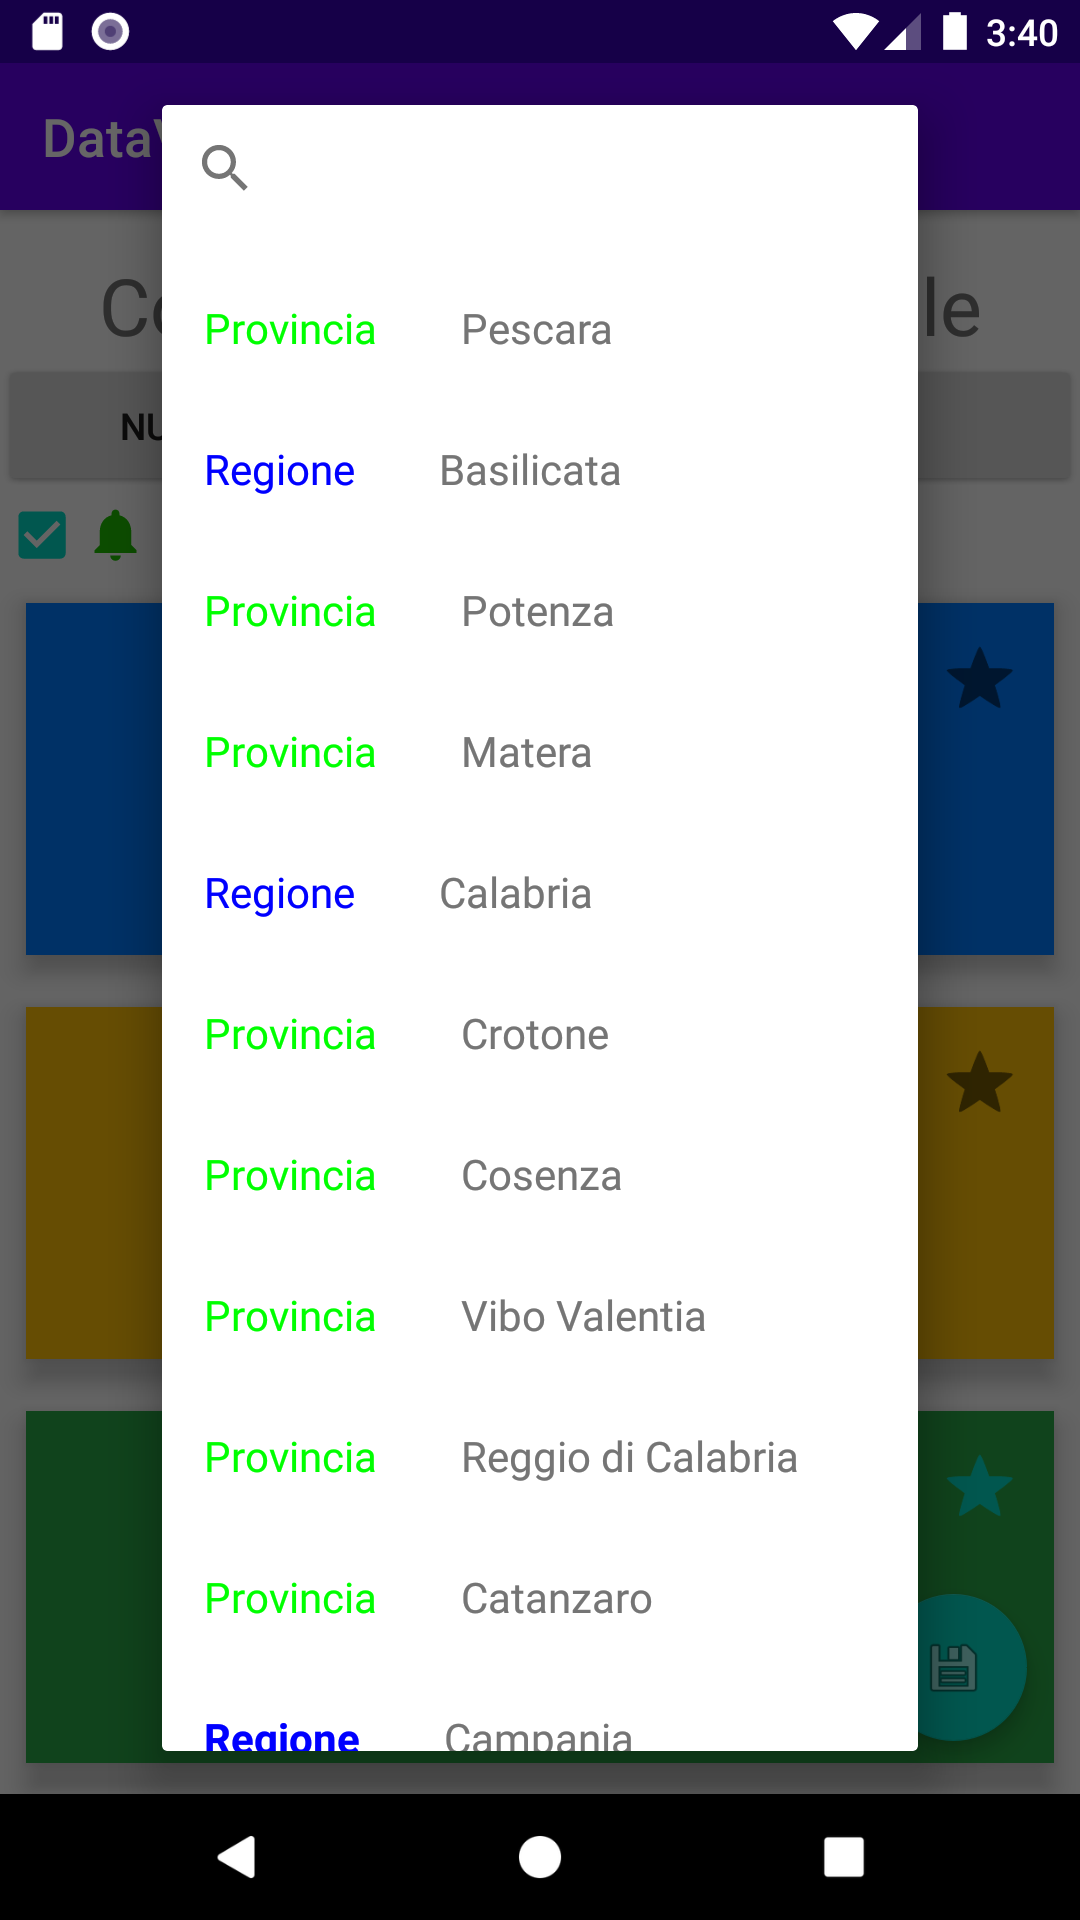
\includegraphics[width=.5\linewidth]{DPC_geo_picker.png}
        \caption{Picker zona geografica}
        \label{fig2}
    \end{figure}

    Grazie al picker (mostrato in figura \ref{fig2}) si puó scegliere la zona geografica di interesse. Puó essere una provincia, una regione oppure si puó selezionare l'andamento nazionale.
    Per comoditá si puó ulteriormente cercare la zona d'interesse premendo sulla \emph{lente d'ingrandimento}.
    Come risultato verranno visualizzati i dati relativi alla zona selezionata.

    \begin{figure}[h]
        \centering
        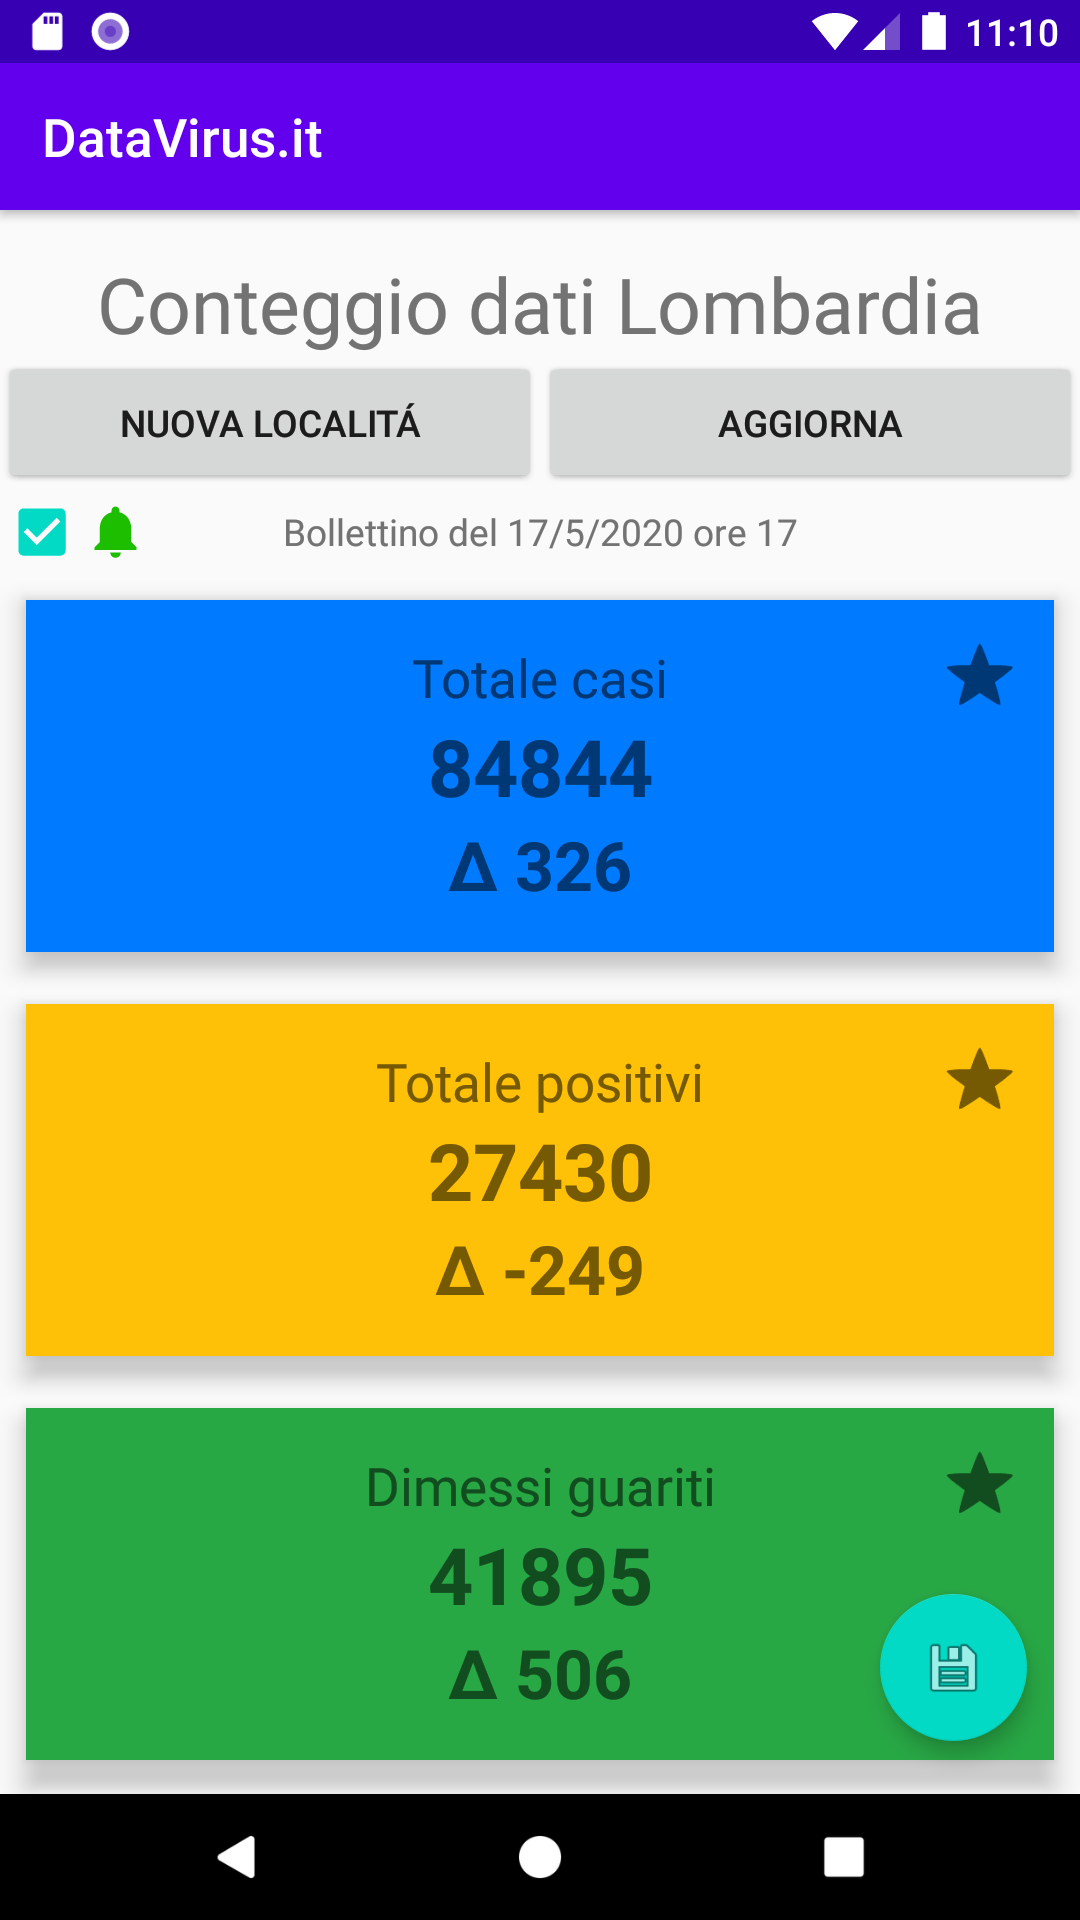
\includegraphics[width=.5\linewidth]{lombardia.png}
        \caption{Esempio visualizzazione regione Lombardia}
        \label{fig3}
    \end{figure}

    Premendo il pulsante back \emph{fisico} si scorreranno all'indietro tutte le selezioni geografiche finora cercate dall'utente. Una volta ritornati alla prima visualizzazione (corrispondente sempre al dato nazionale) l'app si chiuderá.

    \subsection{Implementazione}

    La classe \emph{DPCGeoAdapter} é un'estensione di un DialogFragment che, quando aperto, mostrerá una RecyclerView contenente la lista delle regioni e delle province. 
    \\
    In prima posizione si trova la selezione per il dato nazionale.
    \\
    La lista é strutturata in modo che, per ogni regione, ci sia la lista delle province che la compongono nelle posizioni sottostanti. 
    \\
    Alla pressione di una posizione geografica, il GeoPicker chiamerá la funzione \emph{onDPCGeoClick} di una classe che implementa \emph{OnDPCGeoListener} (nella fattispecie verrá utilizzata la MainActivity).
    L'oggetto passato é di tipo \emph{GeographicElement}, il quale descrive il nome dell'ambito geografico e la sua tipologia (\emph{NAZIONALE, REGIONALE, PROVINCIALE}).

    \section{Preferiti}
    \label{preferiti}
    Ogni tile ha in alto a destra una \emph{stellina}: quando premuta, la tile relativa viene salvata tra i preferiti.
    Per recuperare la lista delle tile salvate é sufficiente premere sul floating button in basso a destra (visibile nella schermata principale dell'app, \ref{fig1:sub2}).

    \begin{figure}[h]
        \centering
        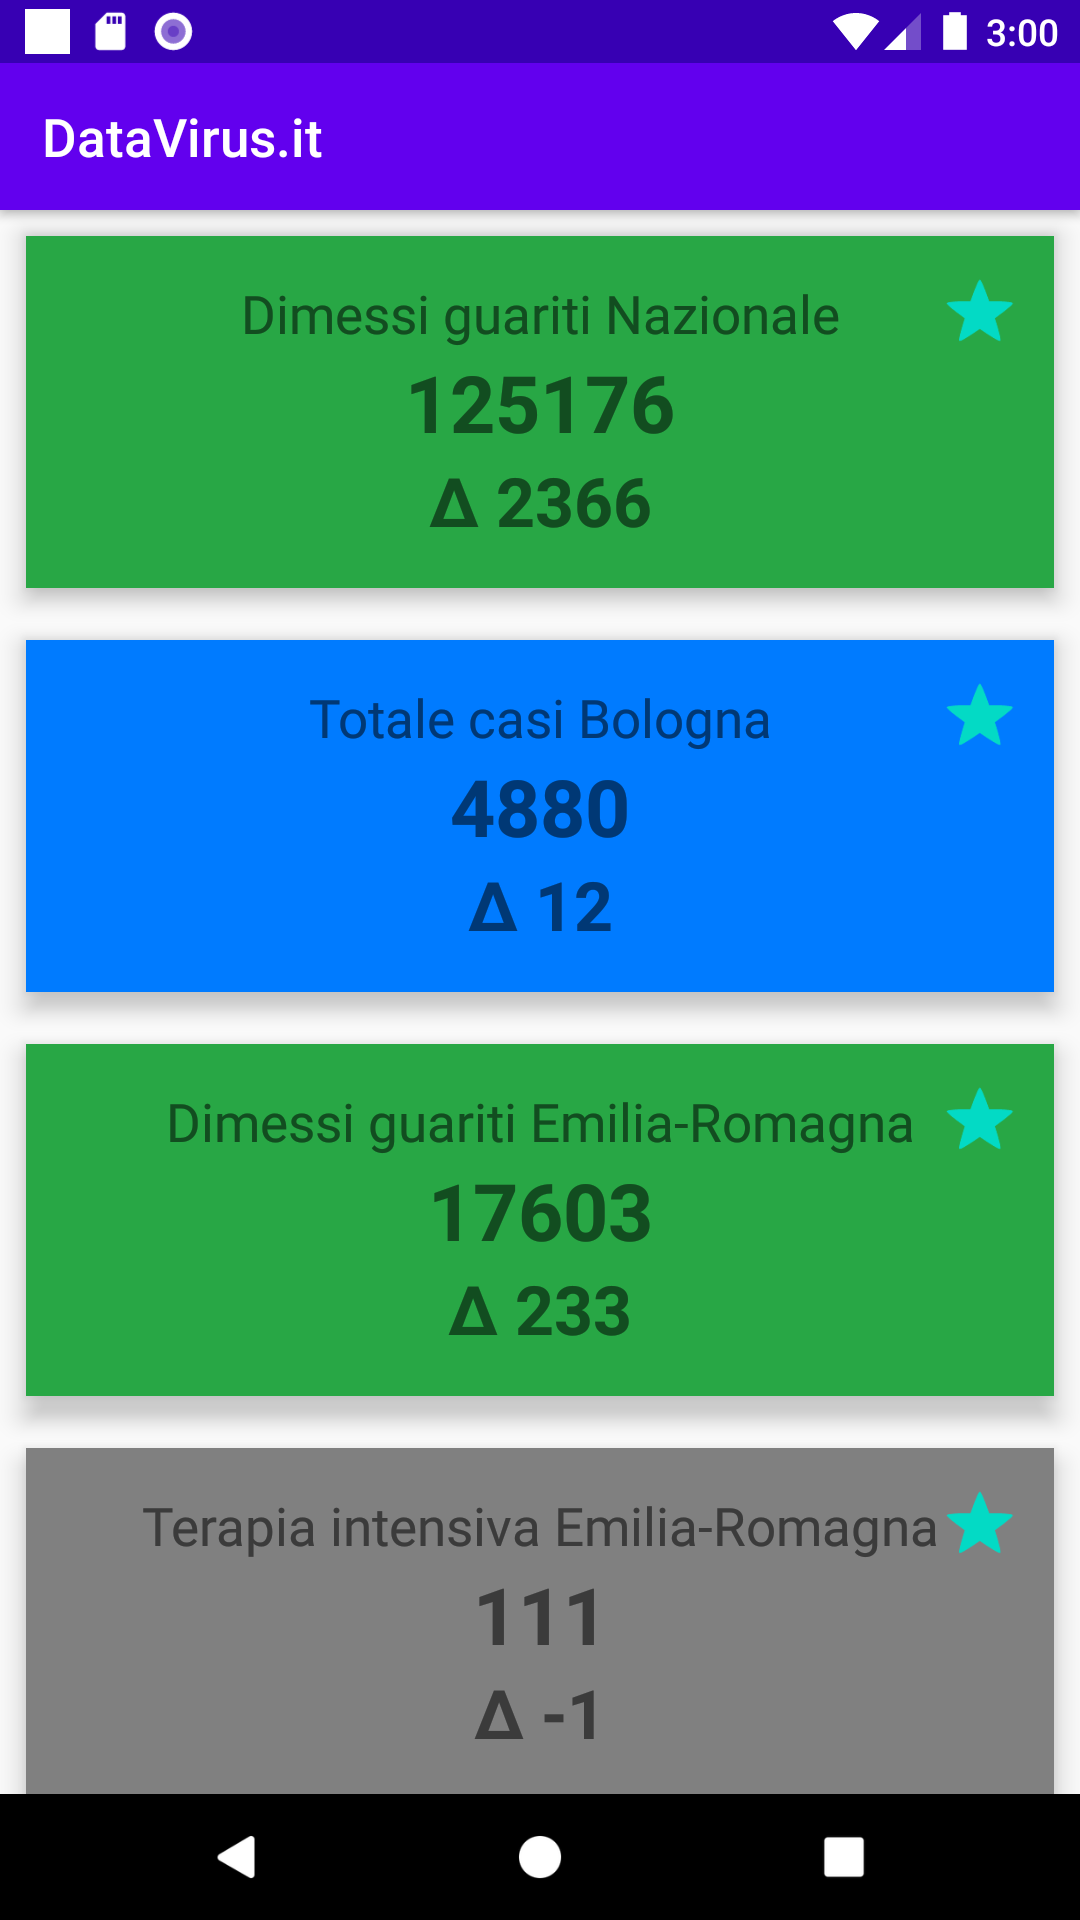
\includegraphics[width=.5\linewidth]{preferences.png}
        \caption{Lista dei preferiti}
        \label{fig4}
    \end{figure}

    Come si puó notare dalla figura \ref{fig4}, le tile salvate sono visualizzate con la loro denominazione geografica a seguito.
    Premendo su una \emph{stellina} precedentemente marcata verrá rimossa tale tile dalla lista dei preferiti.

    \subsection{Implementazione}
    Per il salvataggio dei preferiti si fa uso della classe \emph{ManageStarredTiles}, che offre i metodi per aggiungere o rimuovere un elemento dai preferiti. 
    Per identificare una tile da aggiungere o rimuovere viene passato un oggetto di classe \emph{FieldGeographicElement} (la quale é una estensione della classe \emph{GeographicElement}, con l'ulteriore informazione del parametro del dato di interesse, e.g. \quotes{Totale casi}).
    \\
    I dati sulle tile marcate come starred vengono salvati in un file privato dell'app, in formato JSON. 
    Si é preferito utilizzare il salvataggio dei dati in un file in quanto, in una implementazione futura, il sito web \href{https://datavirus.it}{DataVirus.it} produrrá tale file per i dati preferiti nel formato utilizzato attualmente nell'app.
    \\
    Per la memorizzazione della lista delle tile preferite viene utilizzata la \emph{StarredActivity}, che si occupa di istanziare un \emph{DataTilesFragment} che visualizzerá tutte le tile salvate.
    \\
    Per la visualizzazione della lista delle tile preferite si riutilizza il fragment \emph{DataTilesFragment}.

    \section{Grafici}
    Ogni qualvolta si premerá su una tile, verrá mostrato l'andamento nel tempo del dato selezionato in un grafico.
    Si presenterá la schermata come quella in figura \ref{fig5:sub1}.
    \\
    Il dato che ora viene mostrato puó essere confrontato con altri dati. Per ottenere questo risultato sará sufficiente premere sul pulsante \quotes{+} e selezionare una nuova tile.
    \\
    Ad ogni dato aggiunto viene assegnato un colore random per la sua rappresentazione e apparirá nella lista dei campi attualmente disegnati. 
    Per ciascuno di questi si potrá decidere se nasconderlo o mostrarlo (con la checkbox sulla sinistra) oppure cancellare dalla lista premendo sull'icona del \emph{cestino}.
    \\
    Il grafico é ingrandibile a piacimento, semplicemente utilizzando il \emph{pinch-to-zoom}.

    \begin{figure}[h]
      \centering
      \begin{subfigure}{.5\textwidth}
        \centering
        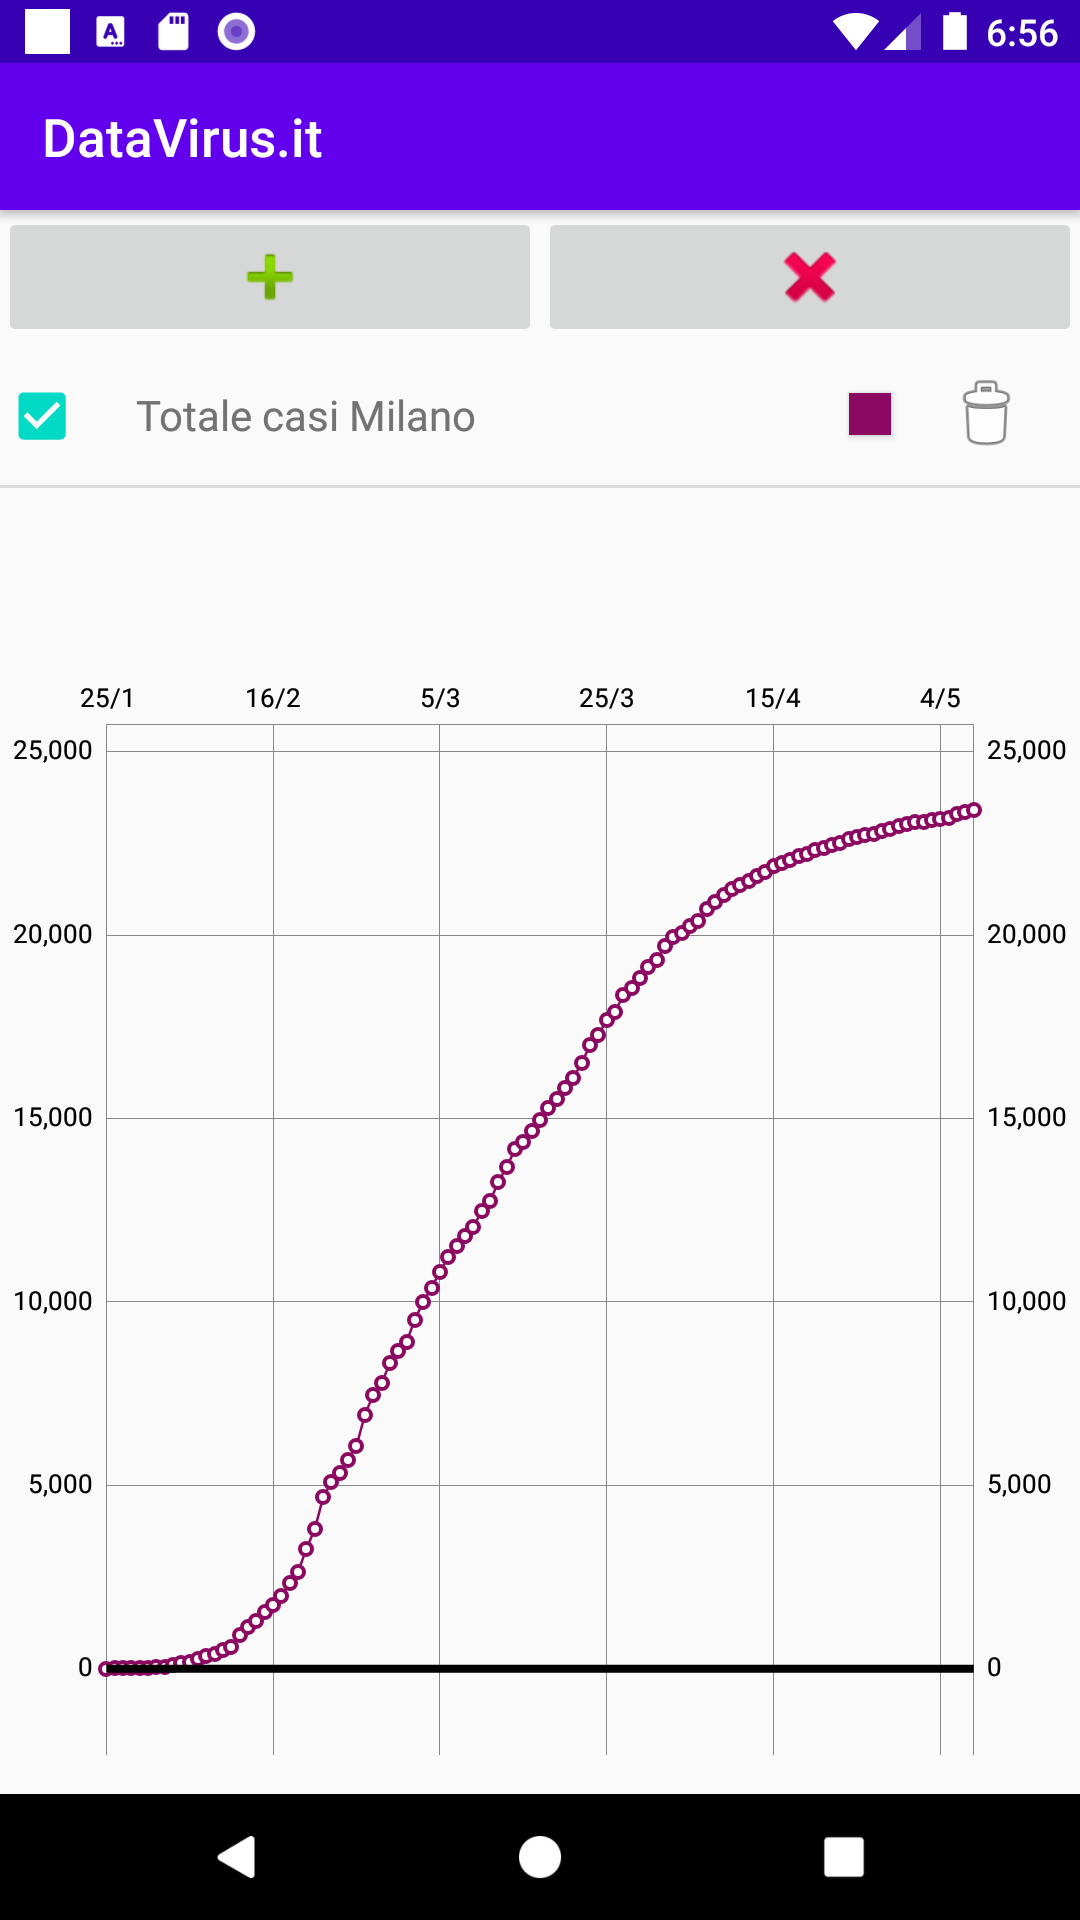
\includegraphics[width=.8\linewidth]{milano.png}
        \caption{Esempio grafico Milano}
        \label{fig5:sub1}
      \end{subfigure}%
      \begin{subfigure}{.5\textwidth}
        \centering
        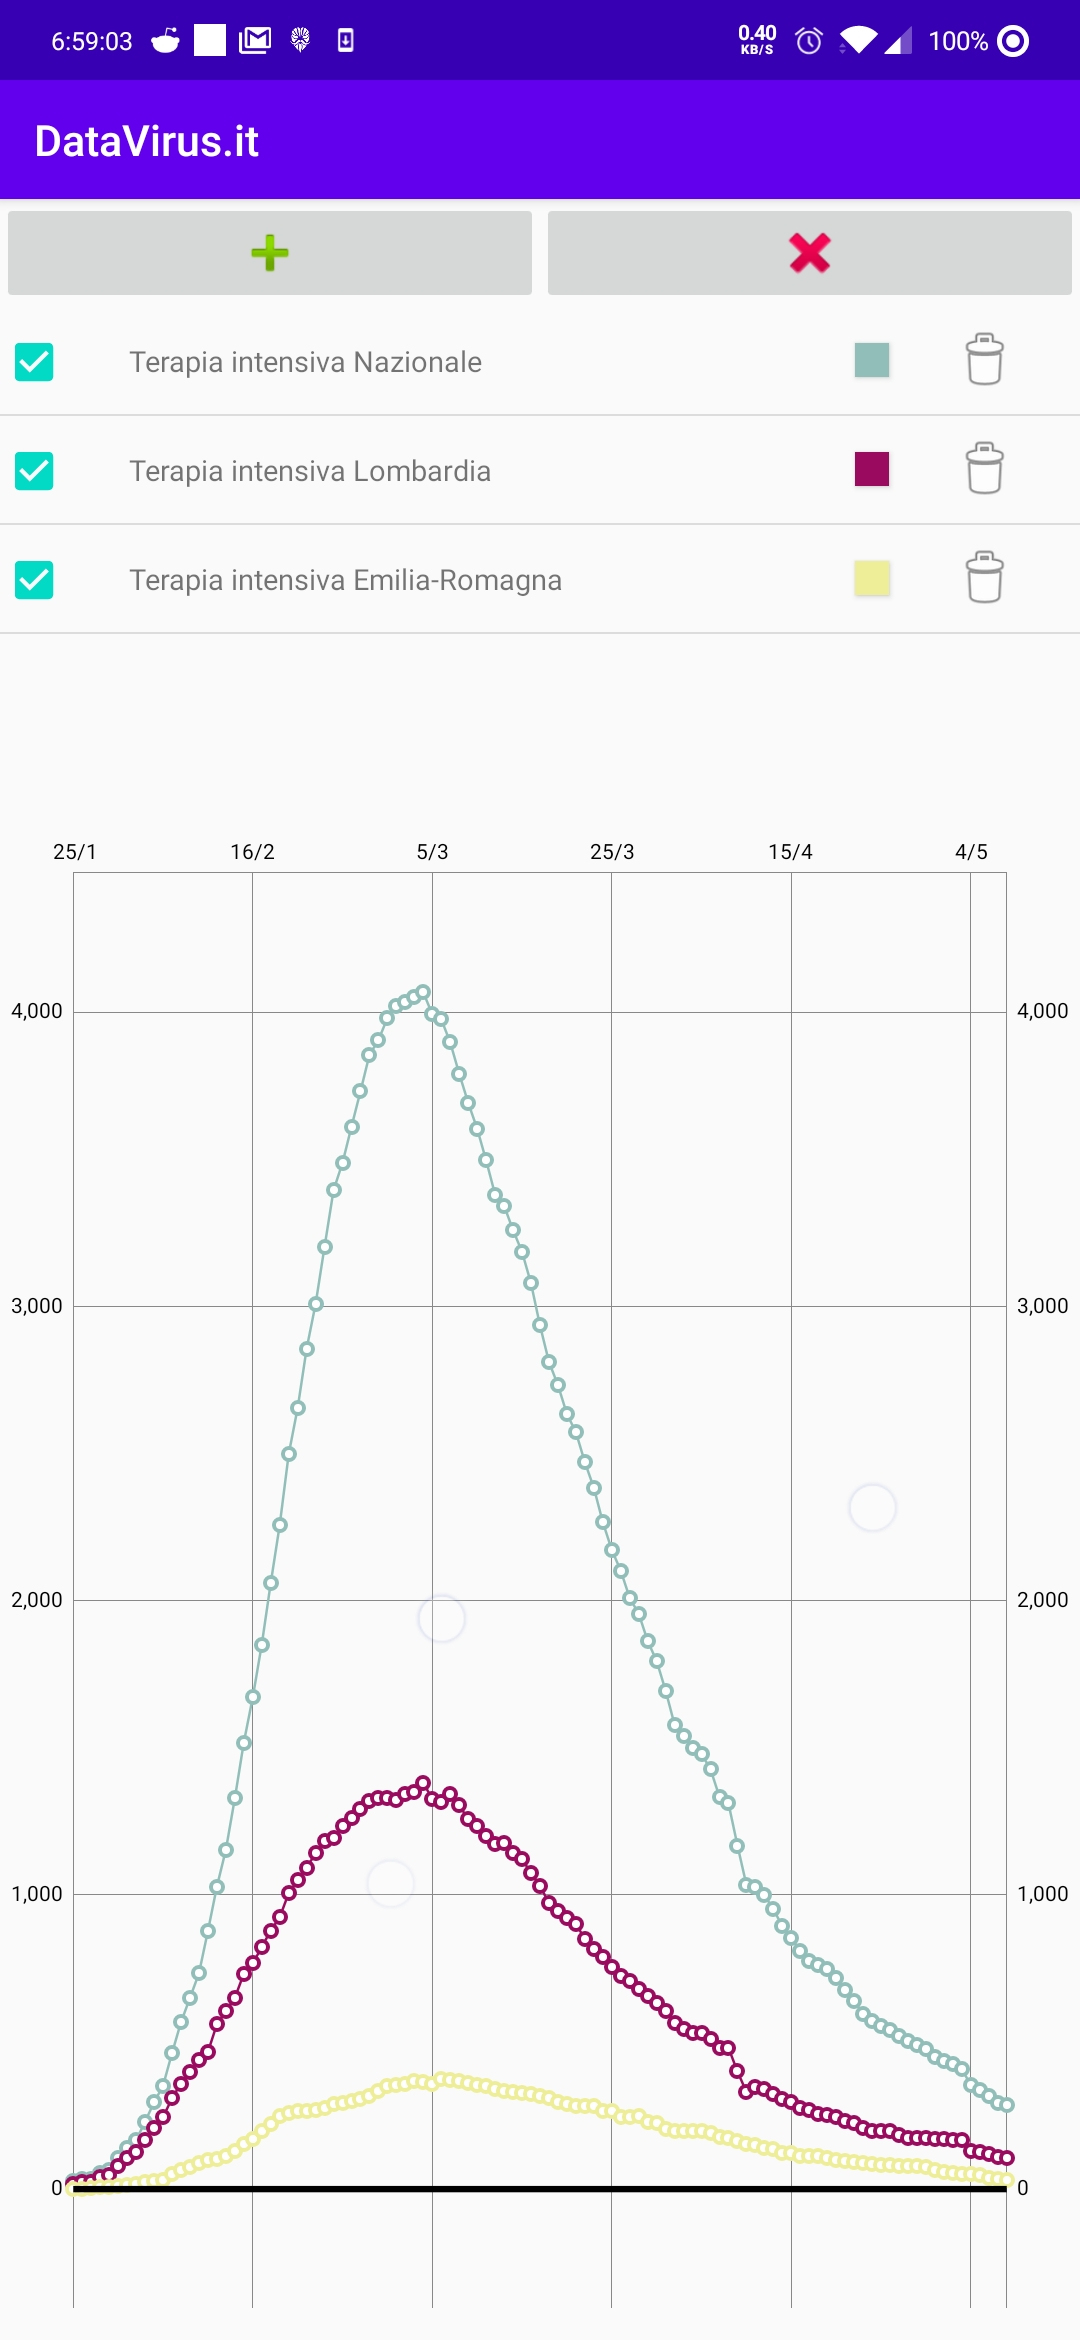
\includegraphics[width=.8\linewidth]{chart_ICU.jpg}
        \caption{Confronto tra terapie intensive}
        \label{fig5:sub2}
      \end{subfigure}
    \end{figure}
    Alla pressione del pulsante \quotes{-} si chiuderá la schermata del grafico e il grafico attualmente disegnato verrá scartato, insieme a tutti i dati precedentemente immessi.
    Il medesimo risultato si puó raggiungere alla pressione del pulsante back \emph{fisico};

    \begin{figure}[h]
      \centering
      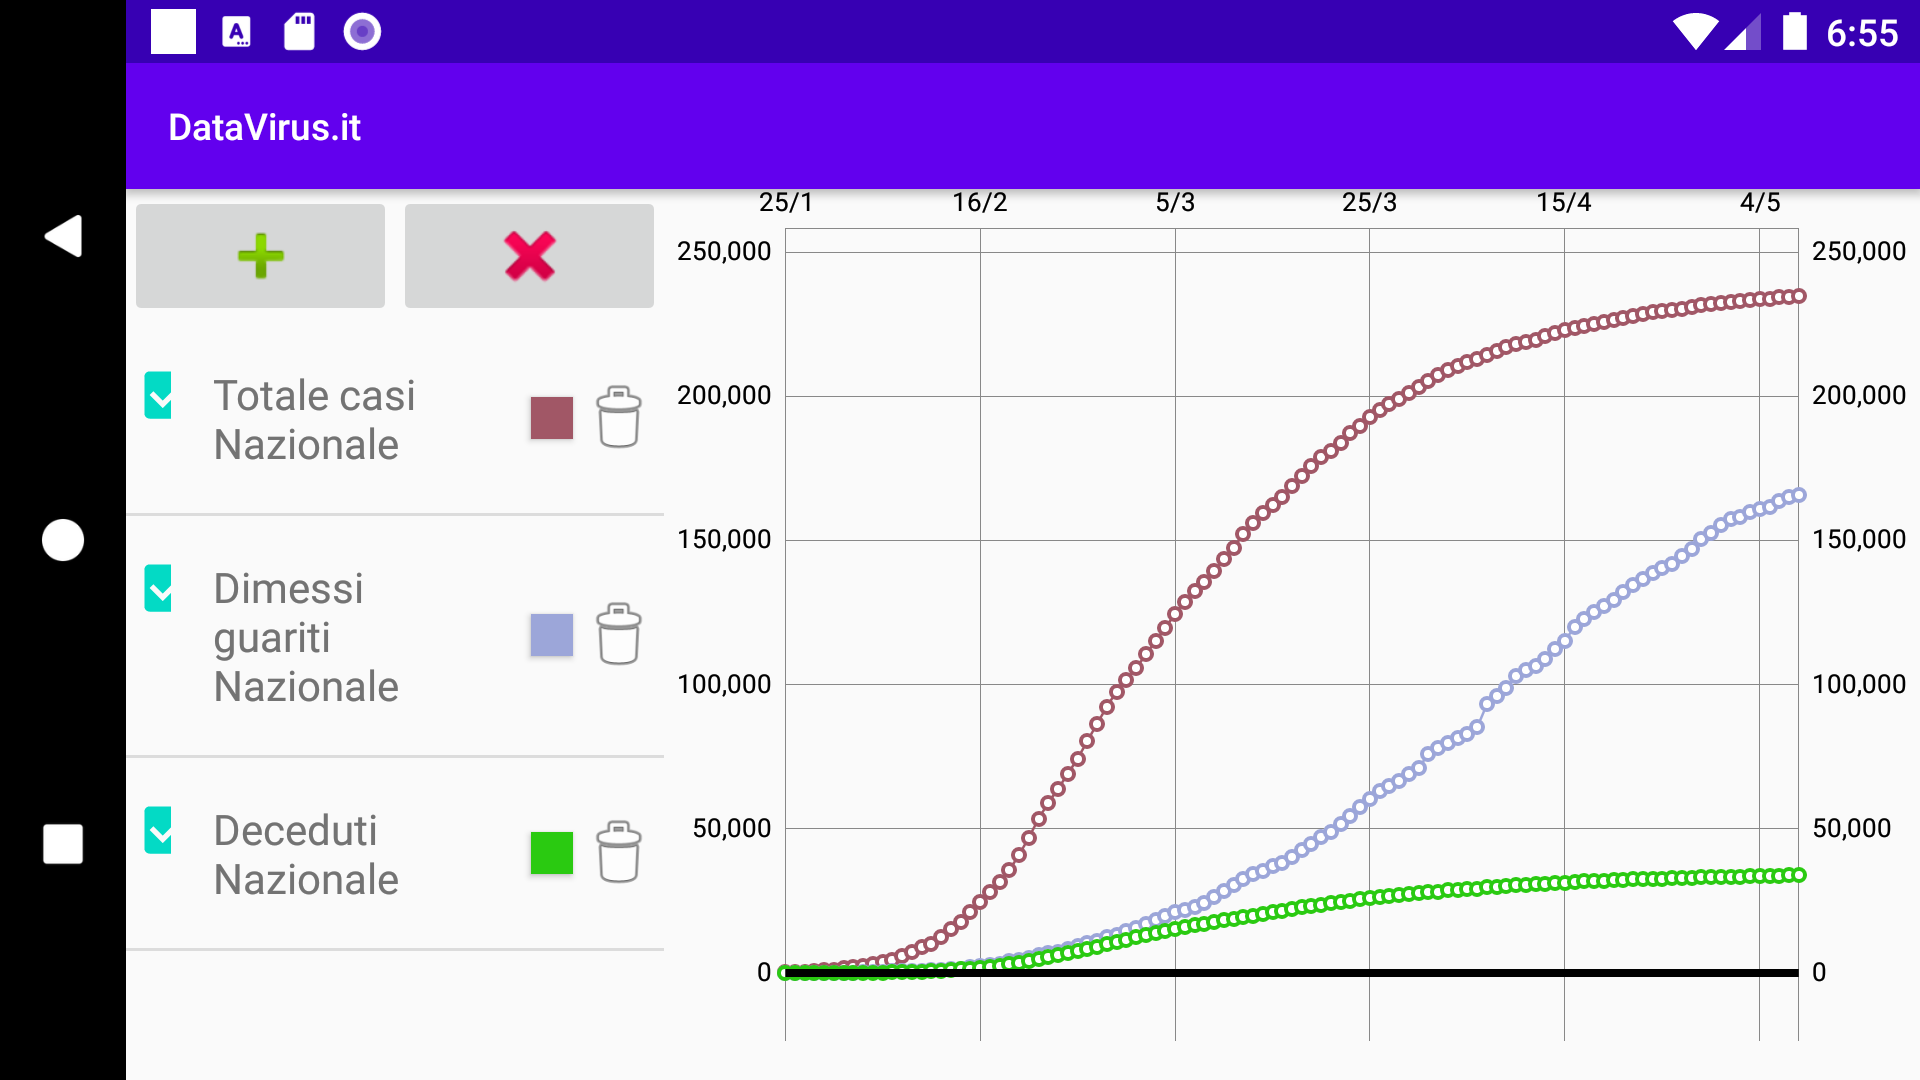
\includegraphics[width=.8\linewidth]{land_chart.png}
      \caption{Visualizzazione landscape della \emph{ChartActivity}}
      \label{fig5a}
    \end{figure}

    Per una maggior comoditá di interazione, é disponibile anche la visualizzazione del grafico con il dispositivo orientato in \emph{landscape} come mostrato in figura \ref{fig5a}

    \subsection{Implementazione}

    Per il grafico é stata utilizzata la libreria \href{https://github.com/PhilJay/MPAndroidChart}{\emph{\textbf{MPAndroidChart}}}, 
    che fornisce un'interfaccia completa per il plotting fornendo molteplici funzionalitá.
    Esistono svariate librerie per disegnare grafici: ho optato per MPAndroidChart perché offre un buon dettaglio ed una semplicitá di implementazione ed utilizzo notevole, senza dover ricorrere a tool a pagamento.
    \\
    Questa viene utilizzata dentro alla \emph{ChartActivity}. I dati sono ottenuti attraverso il singleton \emph{ChartModel}, la quale istanza gestisce i dati da disegnare sul grafico.
    I dati contenuti in \emph{ChartModel} possono essere modificati dall'utente tramite il fragment \emph{ChartElementsList}, che gestisce la RecyclerView contenente tutti gli elementi aggiunti al grafico e le funzionalitá per nascondere il dato oppure rimuoverlo.
    Il pulsante \quotes{+} termina l'activity corrente senza pulire la lista dei dati nel grafico, al contrario del pulsante \quotes{-} che elimina tutti gli elementi finora aggiunti (risultato medesimo quando si preme il pulsante \emph{back} fisico).
    \\
    Quando si preme su una tile si genera l'\emph{intent} per eseguire \emph{ChartActivity}, passando come extra valori gli elementi contenuti in una istanza di \emph{GeographicFieldElement} (estensione di \emph{GeographicElement}).

    \section{Notifiche periodiche}

    Nell'activity principale, a sinistra della data di ultimo aggiornamento, é presente una checkbox con a fianco una campanellina (vedere fig. \ref{fig1:sub2}).
    \\
    Quando marcata, a partire dalle ore 18:00 di ogni giorno, ogni 10 minuti verrá performata una ricerca di nuovi dati aggiornati (orario nel quale il DPC li rende pubblici).
    Nel caso in cui i dati scaricati abbiano data odierna, l'utente verrá avvisato attraverso una notifica. Alla pressione di tale notifica si aprirá l'app. In figura \ref{fig7} un esempio della notifica che verrá mostrata 

    \subsection{Implementazione}
    
    Per gestire le notifiche si é fatto uso di una istanza \emph{DataNotifyReceiver}, classe di tipo \quotes{Broadcast Receiver}
    che alla sua chiamata istanzia un oggetto di tipo \emph{DataParser} (che puó essere richiamato anche senza interfaccia grafica, quindi non mostrando il popup del caricamento) per ottenere dati aggiornati.
    \\
    La chiamata a \emph{DataNotifyReceiver} viene effettuata attraverso un'\emph{intent} performato dall'\emph{AlarmManager}, per impostare l'orario in cui cominciare la ricerca (ore 18:00). 
    La definizione della chiamata all'\emph{AlamrManager} viene eseguita dalla \emph{MainActivity} attraverso i metodi \emph{setAlarm()} ed \emph{unsetAlarm()}.
    \\
    La \emph{MainActivity.setAlarm()} chiama l'\emph{AlarmManager::setInexactRepeating()} passando un intent di esecuzione del BroadcastReceiver \emph{DataNotifyReceiver}, \quotes{puntando} l'orario (inesatto, per motivi di risparmio energetico) delle 6.00PM del giorno successivo 
    (se le ore 18:00 sono giá passate, altrimenti del giorno stesso). 
    La \emph{MainActivity.unsetAlarm()}, come intuibile, disabilita il timer (se questo non é impostato, il comando non produrrá alcun risultato).
    \\
    Nel caso in cui i dati ottenuti dalla repository GitHub siano aggiornati alla data odierna, \emph{DataNotifyReceiver} invia una notifica all'utente (\emph{DataNotifyReceiver.showNotification()}).
    Altrimenti viene impostata l'esecuzione del \emph{DataNotifyReceiver} differita di 10 minuti per una nuova ricerca (con una chiamata al metodo \emph{DataNotifyReceiver.setNextIntent()}).

    \begin{figure}[h]
      \centering
      
\includegraphics[width=.9\linewidth]{notif.jpg}
      \caption{Esempio di notifica}
      \label{fig7}
    \end{figure}

\end{document}